\documentclass[11pt]{article}

\usepackage[margin=1in]{geometry}
\usepackage{graphicx}
\usepackage{booktabs}
\usepackage{amsmath}
\usepackage{xcolor}
\usepackage{caption}
\usepackage{longtable}
\usepackage[colorlinks=true,linkcolor=blue,urlcolor=blue,citecolor=blue]{hyperref}
\usepackage{listings}

\graphicspath{{./}}

\lstset{
  basicstyle=\ttfamily\footnotesize,
  breaklines=true,
  frame=single,
  columns=fullflexible,
  backgroundcolor=\color{gray!8},
}

\newcommand{\code}[1]{\texttt{\small #1}}

\title{\textbf{LLM Perception of Time}\\[2pt]
\large A Seven-Experiment Scoping Study --- Methods, Results, and Reproduction}
\author{Time Project (sandbox exploration)}
\date{Compiled \today\\[4pt]
\small Repository: \code{explorations/time/} \quad Branch: \code{claude/time-project-experiments-g0k16r}}

\begin{document}
\maketitle

\begin{abstract}
\noindent
We ask whether large language models perceive time. The question conflates three distinct
problems, and we separate them with seven controlled, API-only experiments (no training).
\textbf{Self-perception (E1, E2, E5, E6, E10):} a model's apparent ability to estimate its own
generation latency is \emph{entirely a proxy for its own output length}. It is well calibrated
when latency is output-driven (Spearman $\rho=0.79$) and collapses to zero when latency is
driven by hidden reasoning or input prefill ($\rho\approx 0$); estimating in token space beats
seconds ($\rho\,0.89$ vs $0.66$); and the systematic $\sim$2$\times$ length undershoot is mostly
fixable in-context (geometric-mean ratio $0.37\to0.76$) for non-reasoning models.
\textbf{Agency (E3, E4):} agents act on elapsed time only when it is explicit; an
agent's correct time-sensitive decision rate rises from $0.49$ (no signal) to $0.80$ (text
timestamps) to $0.96$ (an explicit harness-injected elapsed-time field). The unifying finding:
\textbf{LLMs have no internal clock --- they have a length estimator, and they respond to
elapsed time only when it is handed to them.} The recurring boundary across the first six
experiments is the \emph{reasoning model}, whose latency hides in tokens it cannot see --- but
E10 sharpens this: reasoning models retain strong \emph{ordinal} awareness of their own effort
(rating $\rho$ up to $0.91$) and fail only at \emph{magnitude}, making the boundary a tractable
calibration problem rather than a wall. Headline numbers carry 95\% bootstrap CIs. This document
is self-contained and reproducible: every number below is regenerated by the committed scripts
from the committed raw data.
\end{abstract}

\tableofcontents

\section{Scope and the three lanes}
\label{sec:scope}

``Does an LLM perceive time?'' is really three questions that are mechanistically unrelated. A
model can be strong at one and hopeless at another:

\begin{enumerate}
  \item \textbf{Temporal reasoning in text} --- ordering events, date arithmetic, durations
  stated in language. Well studied and largely saturated (TimeBench, TRAM, Test-of-Time). We do
  not pursue it.
  \item \textbf{Temporal self-perception} --- can a model estimate the time/length of its
  \emph{own} computation? Experiments E1, E2, E5, E6, E10.
  \item \textbf{Time-aware agency} --- does an agent change behaviour based on elapsed time in
  a transcript? Experiments E3, E4.
\end{enumerate}

The motivation, literature notes and reading list are in \code{research-notes.md}. The
experiment plan is in \code{experiments.md}; the cross-experiment synthesis in
\code{SUMMARY.md}; and an alternative ``train-it-in'' research direction in
\code{direction-train-it-in.md}. This report consolidates all of it.

\section{Shared infrastructure and reproducibility}
\label{sec:infra}

\subsection{Models}
All experiments draw from one fixed roster, defined in \code{common.py}. Exact API model IDs as
used (the study was run on 2026-06-11):

\begin{center}
\begin{tabular}{@{}lllc@{}}
\toprule
Roster key & Provider & API model ID & Reasoning model? \\
\midrule
\code{haiku}      & Anthropic & \code{claude-haiku-4-5-20251001} & no \\
\code{sonnet}     & Anthropic & \code{claude-sonnet-4-6}         & no \\
\code{opus}       & Anthropic & \code{claude-opus-4-8}           & no \\
\code{gpt4o-mini} & OpenAI    & \code{gpt-4o-mini}               & no \\
\code{gpt4o}      & OpenAI    & \code{gpt-4o}                    & no \\
\code{gpt5}       & OpenAI    & \code{gpt-5}                     & yes \\
\code{gpt5.2}     & OpenAI    & \code{gpt-5.2}                   & yes \\
\code{o4-mini}    & OpenAI    & \code{o4-mini}                   & yes \\
\bottomrule
\end{tabular}
\end{center}

Reasoning models spend hidden reasoning tokens, so their wall-clock latency decouples from
visible output. \code{common.py} handles the two provider quirks discovered empirically:
OpenAI reasoning models require \code{max\_completion\_tokens} (not \code{max\_tokens}) and
reject a \code{temperature} argument; \code{claude-opus-4-8} also rejects \code{temperature} in
this harness (so E4 passes \code{temperature=None} for opus). Reasoning models have their token
budget bumped to $\geq 4096$ because hidden reasoning consumes the output budget.

\subsection{The call interface}
Every experiment imports one helper so provider logic is defined once:

\begin{lstlisting}
from common import call            # roster key -> unified call
r = call("sonnet", prompt, max_tokens=1024)
# r: Result(model, text, latency_s, input_tokens, output_tokens, ok, error)
\end{lstlisting}

\code{latency\_s} is wall-clock measured with \code{time.perf\_counter()} around the network
call; it includes network and queueing time, not only generation. Retries use exponential
backoff (4 attempts).

\subsection{Environment}
\begin{itemize}
  \item Python 3.11; virtualenv at \code{explorations/time/.venv}. Pinned dependencies in
  \code{requirements.txt} (anthropic 0.109.1, openai 2.41.1, numpy 2.4.6, pandas 3.0.3,
  scipy 1.17.1, matplotlib 3.10.9).
  \item Secrets via environment variables \code{ANTHROPIC\_API\_KEY} and \code{OPENAI\_API\_KEY}.
\end{itemize}

\subsection{Data format and the resume/dedup scheme}
Each experiment directory \code{eN-*/} contains: \code{run.py} (collect raw data),
\code{analyze.py} (compute statistics and figures), \code{results.jsonl} (one JSON object per
API call), \code{REPORT.md} (self-contained findings), and PNG figures. Collection is
\emph{append-only}; \code{run.py} is idempotent via a \code{load\_done()} check on a logical key
(typically \code{(model, task/scenario, trial, condition)}), so an interrupted run resumes
without recomputation.

\paragraph{Known hazard (documented, not silent).} This append + \code{load\_done()} scheme is
\textbf{not safe against concurrent writers}: two \code{run.py} processes for the same
experiment will both pass \code{load\_done()} and write duplicate rows. This actually occurred
during the run (see \S\ref{sec:process}). The fix is \code{dedup.py}, which canonicalizes each
\code{results.jsonl} by its logical key (keeping the last occurrence) before analysis.
\code{analyze.py} scripts also tolerate duplicates, but \code{dedup.py} guarantees exact counts.

\subsection{How to reproduce}
\label{sec:reproduce}
From \code{explorations/time/}:
\begin{lstlisting}
python -m venv .venv && . .venv/bin/activate
pip install -r requirements.txt
export ANTHROPIC_API_KEY=...  OPENAI_API_KEY=...

# Re-derive every table and figure from the committed raw data (no API calls):
for d in e1-self-duration e2-token-time e3-log-gap-probe \
         e4-harness-clock e5-latency-decoupled e6-length-bias \
         e10-reasoning-tokens; do
  ( cd $d && python analyze.py )
done

# To re-collect raw data (spends API budget). run.py RESUMES from results.jsonl,
# so for a true from-scratch run, move the existing file aside first:
#   cd eN-*
#   mv results.jsonl results.jsonl.bak        # keep a backup; run.py starts fresh
#   python run.py                             # collect; resumable if interrupted
#   python ../dedup.py eN-*                   # only needed if writers ran concurrently
# Quick smoke test of one model/task without a full sweep:  python run.py dryrun
# Collection knobs (model ROSTER, N_TRIALS) are at the top of each eN-*/run.py.
\end{lstlisting}
Re-running \code{analyze.py} on the committed \code{results.jsonl} reproduces every statistic in
this report exactly. Re-collecting with \code{run.py} reproduces them up to sampling noise.

\subsection{Determinism caveats}
Calls use provider-default temperature (not pinned), so re-collection varies trial-to-trial.
Absolute wall-clock numbers are harness- and hardware-specific. We therefore lead with
\emph{rank} statistics (Spearman $\rho$, ordering accuracy) and \emph{between-condition}
contrasts, which are robust, and treat absolute latencies as distributions (multiple trials,
reported coefficient of variation) rather than points.

\section{E1 --- Self-duration calibration}
\label{sec:e1}
\textbf{Question.} Can a model estimate its own wall-clock generation time?
\textbf{Hypothesis (from the literature).} No: estimates overshoot by 4--7$\times$ and ordering
is at chance.

\paragraph{Setup.} 12 tasks spanning short$\to$long outputs. For each (model $\times$ task
$\times$ 3 trials): a \textsc{pre} estimate (``how many seconds will your response take?''), the
real generation (record \code{latency\_s}, \code{output\_tokens}), and a \textsc{post} estimate
(``how long did that take?''). 6 models, 648 calls, 216 units.

\paragraph{Results (Table~\ref{tab:e1}, Fig.~\ref{fig:e1}).} The hypothesis is \emph{rejected}
for this task set. Estimate/actual geometric-mean ratios sit near 1 (overall 0.81), not
4--7$\times$; ordering accuracy is 0.79--0.95 (chance $=0.5$); Spearman $\rho_{\textsc{pre}}$ is
0.74--0.94, all $p<0.001$. Trial-to-trial latency noise is small (median CV 0.04--0.14), so the
calibration signal is real.

\begin{table}[h]
\centering
\caption{E1: per-model calibration. Ratio is geometric-mean estimate/actual.}
\label{tab:e1}
\begin{tabular}{@{}lcccc@{}}
\toprule
model & gm ratio \textsc{pre} & $\rho_{\textsc{pre}}$ & ordering acc. & $\rho_{\textsc{post}}$ \\
\midrule
opus       & 0.93 & 0.94 & 0.94 & 0.95 \\
sonnet     & 0.76 & 0.85 & 0.95 & 0.85 \\
gpt4o      & 1.04 & 0.83 & 0.86 & 0.77 \\
gpt4o-mini & 1.36 & 0.74 & 0.86 & 0.89 \\
haiku      & 0.86 & 0.89 & 0.88 & 0.76 \\
gpt5.2     & 0.32 & 0.74 & 0.79 & 0.84 \\
\midrule
\textbf{overall} & \textbf{0.81} & \textbf{0.75} & --- & --- \\
\bottomrule
\end{tabular}
\end{table}

\begin{figure}[h]
\centering
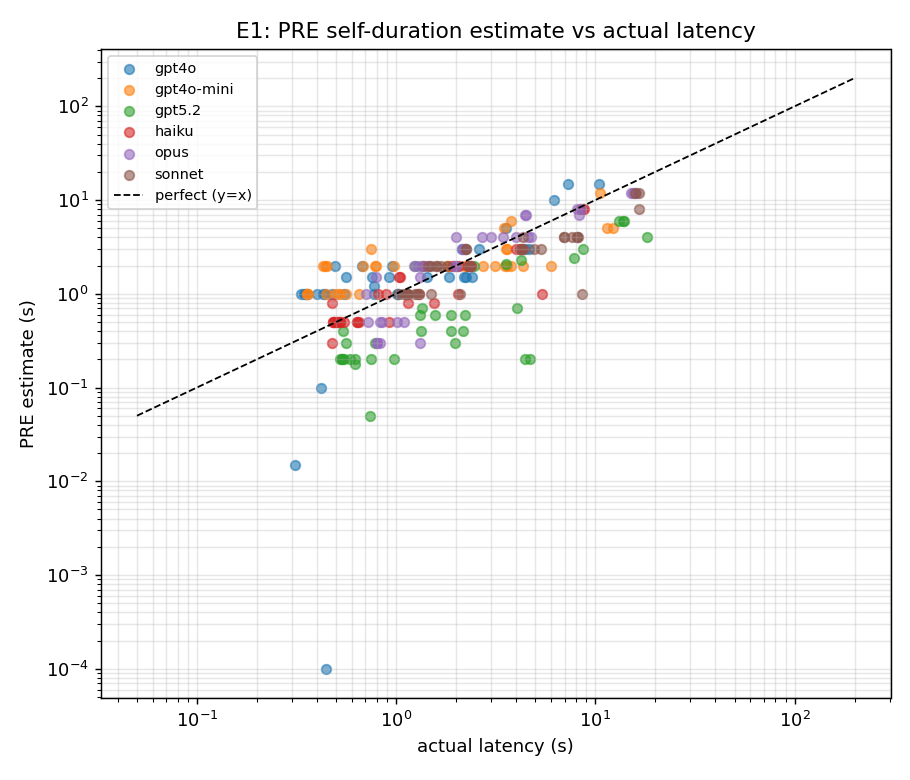
\includegraphics[width=0.62\textwidth]{e1-self-duration/fig_scatter.png}
\caption{E1: estimated vs.\ actual latency (log--log), pooled. Tight diagonal structure ---
models rank and roughly size their own latency.}
\label{fig:e1}
\end{figure}

\paragraph{Why the contradiction.} The task set varies tasks primarily by \emph{output length},
and for non-reasoning models latency is output-token--dominated. Models can anticipate roughly
how long their own output will be, so they predict latency well via an implicit length proxy ---
not via a clock. Two tells: gpt5.2 (reasoning) is the worst calibrated (0.32$\times$, it
undershoots because hidden reasoning latency is invisible), and undershoots cluster on
free-form generations (\code{code}, \code{story}). E5 (\S\ref{sec:e5}) confirms this mechanism
and reconciles the result with the literature.

\paragraph{Verdict.} Rejected \emph{for this regime}: models predict their own latency well when
it is output-driven ($\rho$ up to 0.94), via a length proxy, not a clock.

\section{E2 --- Token/step proxy vs second-space}
\label{sec:e2}
\textbf{Hypothesis.} Output length is something the model has more access to than time, so
estimating in tokens should be better-calibrated than in seconds.

\paragraph{Setup.} Same task family. Four conditions per (model$\times$task$\times$3): (a) predict
seconds; (b) predict output tokens; (c) predict tokens then convert via a measured per-model
tokens/sec constant; (d) reason about size first, then predict seconds. 6 models, 864 calls.

\paragraph{Results (Table~\ref{tab:e2}, Fig.~\ref{fig:e2}).} Token-space beats second-space:
pooled $\rho\,0.889$ vs $0.657$ ($\Delta=+0.231$). Per-model, seconds estimates correlate well
\emph{within} a model but the scale is wildly model-specific (gpt4o-mini overshoots 6.6$\times$,
o4-mini undershoots 0.5$\times$), which destroys the pooled correlation; tokens normalize this.
Models under-predict their own length $\sim$2$\times$ (token ratio 0.49). Converting tokens to
seconds (c) compounds the undershoot (0.24). Reasoning first (d) does \emph{not} help (0.545).

\begin{table}[h]
\centering
\caption{E2: pooled calibration by estimation condition.}
\label{tab:e2}
\begin{tabular}{@{}lcc@{}}
\toprule
condition & $\rho$ (pred vs actual) & gm(pred/actual) \\
\midrule
(a) seconds          & 0.657 & 2.16 \\
(b) tokens           & \textbf{0.889} & 0.49 \\
(c) tokens$\to$sec   & 0.829 & 0.24 \\
(d) reason-then-sec  & 0.545 & 1.08 \\
\bottomrule
\end{tabular}
\end{table}

\begin{figure}[h]
\centering
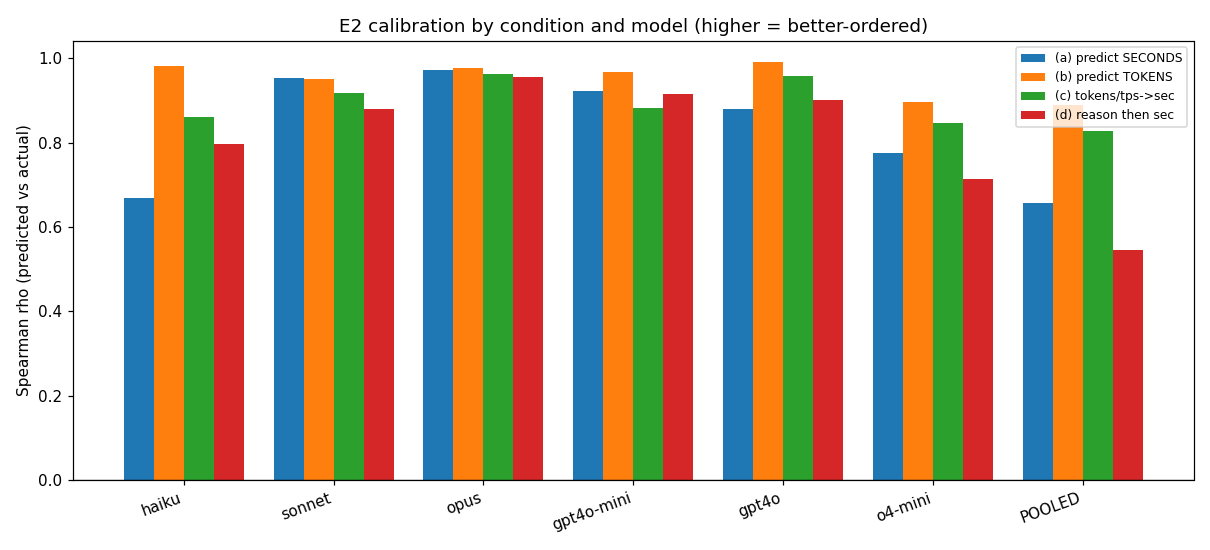
\includegraphics[width=0.7\textwidth]{e2-token-time/rho_by_condition.png}
\caption{E2: rank correlation of estimate vs.\ actual, by condition and model. Token space
(b) is uniformly high; second space (a) and reasoning (d) are noisier.}
\label{fig:e2}
\end{figure}

\paragraph{Verdict.} Supported. Models track their own output length, not time; the practical
target for any self-estimation is token/step space plus a bias correction for the
$\sim$2$\times$ undershoot. The approach fails for reasoning models (o4-mini token ratio 0.10),
the recurring boundary.

\section{E3 --- Log-gap probe (are agents timestamp-blind?)}
\label{sec:e3}
\textbf{Hypothesis.} Agents are blind to elapsed time encoded in a transcript: varying only the
timestamp gap will not flip a time-sensitive decision.

\paragraph{Setup.} 9 scenarios (stock price, weather, inventory, 2FA code, session token,
``wait a bit'', geocode, medication dose, food safety), each a short transcript where an action
happened at $t_0$ and a decision is needed at $t_0+\text{gap}$. The transcript is held
\emph{fixed}; only the gap varies over \{1s, 1min, 1h, 1day, 1week\}, plus a no-timestamp
control. Each scenario declares a human-sensible staleness threshold. One-word forced decision.
5 models, 810 calls. We separate \emph{sensitivity} (does the decision respond to the gap at
all?) from \emph{correctness} (does it flip at the right threshold?).

\paragraph{Results (Table~\ref{tab:e3}, Fig.~\ref{fig:e3}).} Blindness is \emph{graded, not
binary}. Sensitivity scales with model strength (opus 1.00 $\to$ haiku 0.56); when models do
attend they are well calibrated (correctness 0.80--0.93). Stripping timestamps (control) changes
the decision for no model except opus (33\%). The deficit is \emph{attention to the clock}, not
temporal judgement.

\begin{table}[h]
\centering
\caption{E3: sensitivity and correctness by model.}
\label{tab:e3}
\begin{tabular}{@{}lcc@{}}
\toprule
model & sensitivity & correctness \\
\midrule
opus   & 1.00 & 0.86 \\
sonnet & 0.78 & 0.93 \\
gpt5.2 & 0.78 & 0.89 \\
gpt4o  & 0.67 & 0.80 \\
haiku  & 0.56 & 0.82 \\
\bottomrule
\end{tabular}
\end{table}

\begin{figure}[h]
\centering
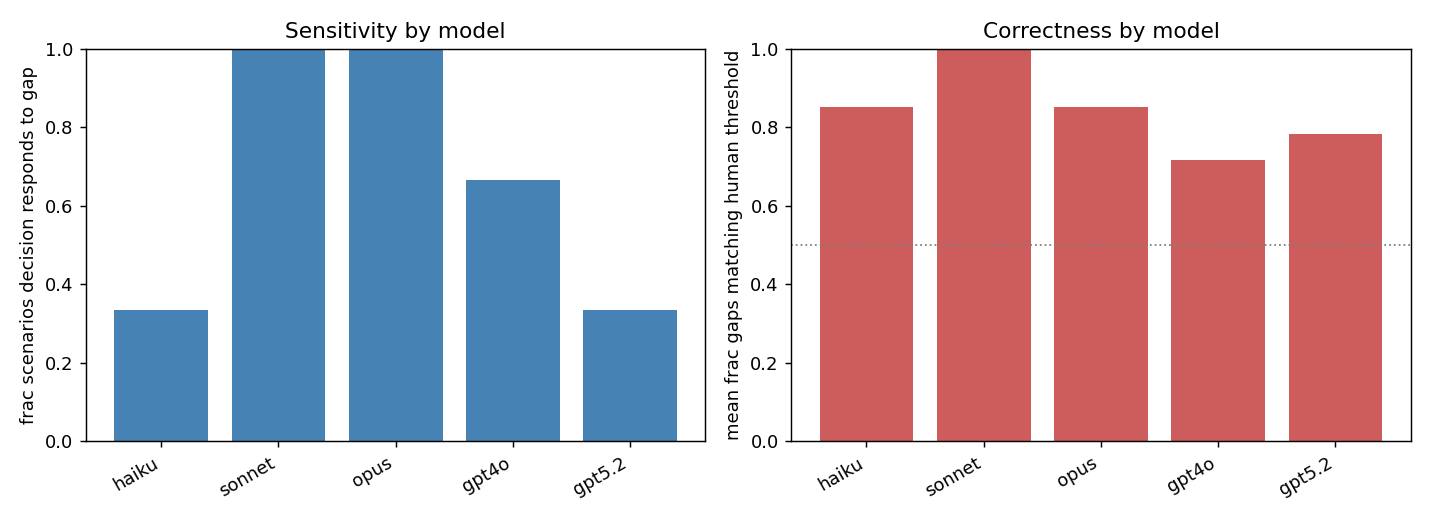
\includegraphics[width=0.72\textwidth]{e3-log-gap-probe/sensitivity.png}
\caption{E3: per-scenario sensitivity by model (does the decision change across the gap
ladder?). opus reads the clock everywhere; weaker models flatten on extreme-threshold
scenarios.}
\label{fig:e3}
\end{figure}

\paragraph{Verdict.} Partially supported, and it refines TicToc's near-random framing: with a
clean single-variable manipulation, strong models \emph{do} respond to gaps and are calibrated;
the weak link is inconsistent attention to the clock.

\section{E4 --- Harness clock (sensor vs text timestamps)}
\label{sec:e4}
\textbf{Hypothesis.} Much ``temporal blindness'' is a missing sensor: an explicit
harness-injected elapsed-time field beats burying timestamps in text.

\paragraph{Setup.} E3-family time-sensitive decisions under three presentation conditions of the
\emph{same} scenario+gap: (a) no time signal; (b) absolute timestamps in the transcript text
(model must compute the gap); (c) an explicit harness field, e.g.\
\code{[elapsed since last action: 3 hours 12 minutes]}. Gaps straddle each threshold so a correct
decision is well defined. 5 models, 1620 calls, 0 failures.

\paragraph{Results (Table~\ref{tab:e4}, Fig.~\ref{fig:e4}).} The harness clock wins decisively.
Correct-decision rate: 0.494 (none) $\to$ 0.796 (text) $\to$ 0.956 (harness). Text over nothing
$=+0.302$; harness over text $=+0.159$; harness over nothing $=+0.461$. The lift is largest for
weak models and smallest for the reasoning model (o4-mini already computes gaps from text). The
cleanest effect is on the fresh side of the threshold, where no-signal models default to
``stale'' (fresh accuracy 0.23) and the harness clock nearly fixes it (0.94).

\begin{table}[h]
\centering
\caption{E4: correct-decision rate by presentation condition (n=540 each).}
\label{tab:e4}
\begin{tabular}{@{}lc@{}}
\toprule
condition & correct-decision rate \\
\midrule
(a) no time signal     & 0.494 \\
(b) text timestamps    & 0.796 \\
(c) harness clock      & \textbf{0.956} \\
\bottomrule
\end{tabular}
\end{table}

\begin{figure}[h]
\centering
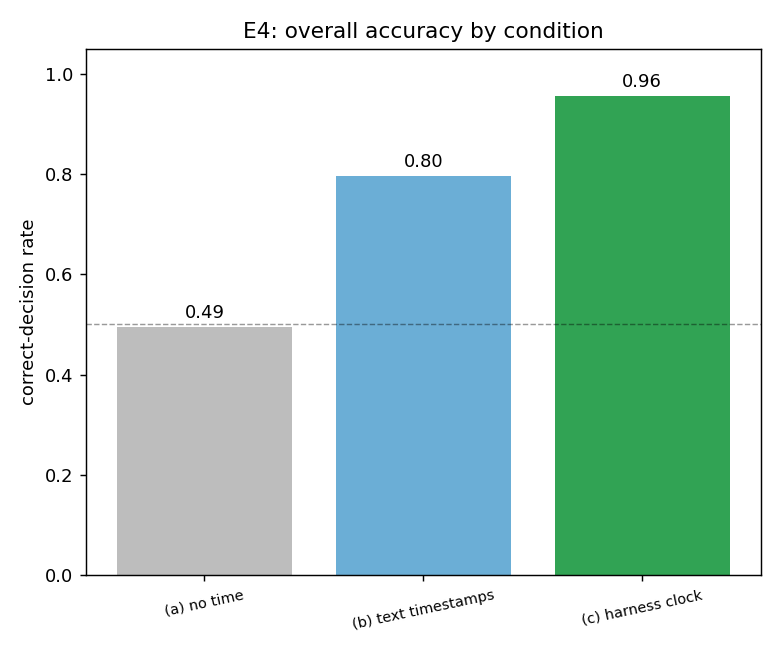
\includegraphics[width=0.6\textwidth]{e4-harness-clock/fig_overall_by_condition.png}
\caption{E4: overall correct-decision rate by condition. The sensor (c) closes most of the gap
left by text timestamps (b).}
\label{fig:e4}
\end{figure}

\paragraph{Verdict.} Supported. A large share of agent temporal blindness is a missing-sensor /
tooling problem, addressable at the harness layer without post-training. \emph{Caveat:} the
prompt states the staleness rule, so this isolates the \emph{sensor}, not threshold knowledge;
the between-condition contrast is the result, not the absolute accuracies (which are optimistic).

\section{E5 --- Latency-decoupled probe (the linchpin validity check)}
\label{sec:e5}
\textbf{Hypothesis.} E1/E2's calibration is a pure output-length proxy: it should survive when
latency is output-driven and \emph{collapse} when latency is decoupled from output length.

\paragraph{Setup.} Three task families, all logging a \textsc{pre} seconds-estimate and actual
latency: \textbf{Type~A (reasoning-decoupled)} --- short fixed output, varying difficulty
($2{+}2$ \ldots derangement of 8); latency varies via hidden reasoning. \textbf{Type~B
(input-decoupled)} --- output pinned to one word, input filler varied 100$\to$30\,000 tokens;
latency varies via prefill. \textbf{Type~C (output-driven control)} --- output length varies.
5 models, 450 calls.

\paragraph{Results (Table~\ref{tab:e5}, Fig.~\ref{fig:e5}).} The prediction holds decisively.
Control (C) is strongly calibrated ($\rho\,0.788$, $p<0.001$), but the reasoning-decoupled (A)
and input-decoupled (B) families collapse to no significant correlation \emph{despite} 16$\times$
and 9$\times$ actual-latency spreads. Even reasoning models fail Type~A (gpt5.2 $\rho\,0.30$ n.s.,
o4-mini $-0.36$ n.s.). The mechanism is legible in Type~B: models emit a near-\emph{constant}
time estimate as input grows --- e.g.\ haiku \code{[1.0, 1.0, 1.3, 1.0]} seconds for inputs of
100/1k/8k/30k tokens while actual latency rises \code{[0.52, 0.59, 0.71, 0.97]}; o4-mini emits
\code{[1.0, 1.0, 1.0, 1.0]}. A 300$\times$ change in input length moves the estimate not at all.

\begin{table}[h]
\centering
\caption{E5: pooled $\rho$(estimate, actual latency) by task type.}
\label{tab:e5}
\begin{tabular}{@{}lccc@{}}
\toprule
type & pooled $\rho$ & gm(est/act) & actual-latency spread \\
\midrule
C --- output-driven (control)   & \textbf{0.788} & 1.30 & 61.9$\times$ \\
A --- reasoning-decoupled       & $-0.067$ (n.s.) & 2.01 & 16.2$\times$ \\
B --- input-decoupled           & $-0.231$ (n.s.) & 1.44 & 8.9$\times$ \\
\bottomrule
\end{tabular}
\end{table}

\begin{figure}[h]
\centering
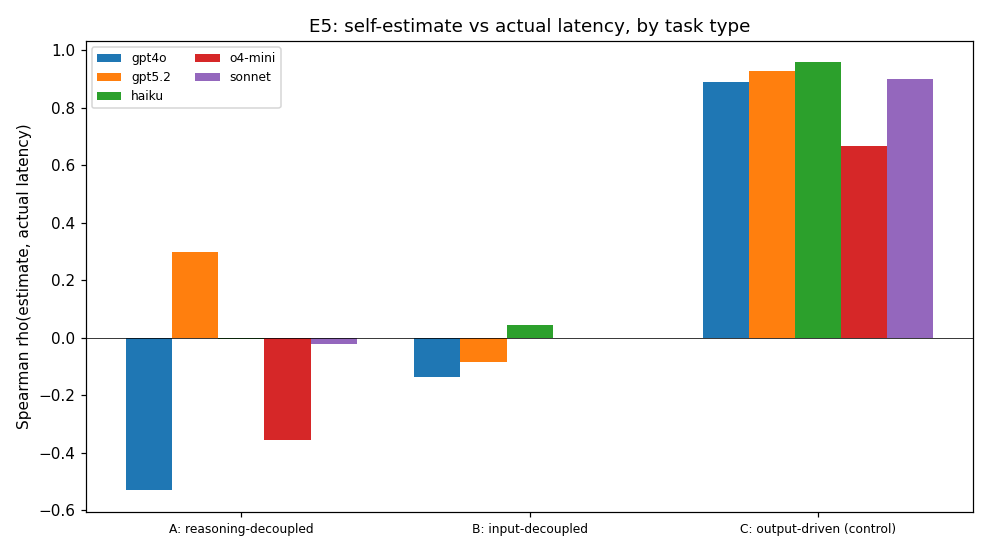
\includegraphics[width=0.62\textwidth]{e5-latency-decoupled/rho_by_type.png}
\caption{E5: self-estimate vs.\ actual latency by task type and model. Calibration exists only
in the output-driven control (C); it vanishes once latency is decoupled (A, B).}
\label{fig:e5}
\end{figure}

\paragraph{Reconciliation.} This resolves E1's apparent contradiction of the literature. There
is no contradiction: in length-dominated tasks models look calibrated; in latency-decoupled
tasks (closer to what negative-result papers used) they are blind, exactly as reported. The
regime is the hidden variable, and E5 makes it explicit.

\paragraph{Verdict.} Confirmed. Self-latency calibration is a pure output-length proxy; any
``train-it-in'' effort must target the latency the model currently cannot see (reasoning tokens,
prefill), not output length.

\section{E6 --- Length-estimation bias correction}
\label{sec:e6}
\textbf{Hypothesis.} The $\sim$2$\times$ output-length undershoot (E2) closes with in-context
interventions, no training.

\paragraph{Setup.} 10 length-varying tasks. Per (model$\times$task$\times$3): one generation
(actual tokens) and three estimate conditions --- \textbf{bare} (E2 baseline), \textbf{anchors}
(few-shot token-count calibration table), \textbf{self\_revise} (predict, then ``you tend to
under-count, adjust'', then \code{FINAL: <n>}). 6 models, 720 calls.

\paragraph{Results (Table~\ref{tab:e6}, Fig.~\ref{fig:e6}).} In-context calibration substantially
closes the bias while keeping ranking intact. Pooled gm(pred/actual) moves $0.37$ (bare,
$\approx 2.7\times$ undershoot) $\to 0.55$ (anchors) $\to 0.76$ (self-revise), with $\rho$
holding near 0.83. Per-model nuance is the real story: strong models land near 1.0 under
self-revision (opus 0.82, sonnet 0.78), weak models \emph{overcorrect} (haiku $\to 2.01$,
overshoot), and o4-mini stays stuck (0.08$\to$0.19).

\begin{table}[h]
\centering
\caption{E6: pooled length-estimate calibration by condition (1.0 = perfect; $<$1 = undershoot).}
\label{tab:e6}
\begin{tabular}{@{}lccc@{}}
\toprule
condition & pooled gm(pred/act) & $\Delta$ vs bare & pooled $\rho$ \\
\midrule
bare        & 0.37 & ---    & 0.842 \\
anchors     & 0.55 & $+0.18$ & 0.861 \\
self\_revise & \textbf{0.76} & $+0.39$ & 0.825 \\
\bottomrule
\end{tabular}
\end{table}

\begin{figure}[h]
\centering
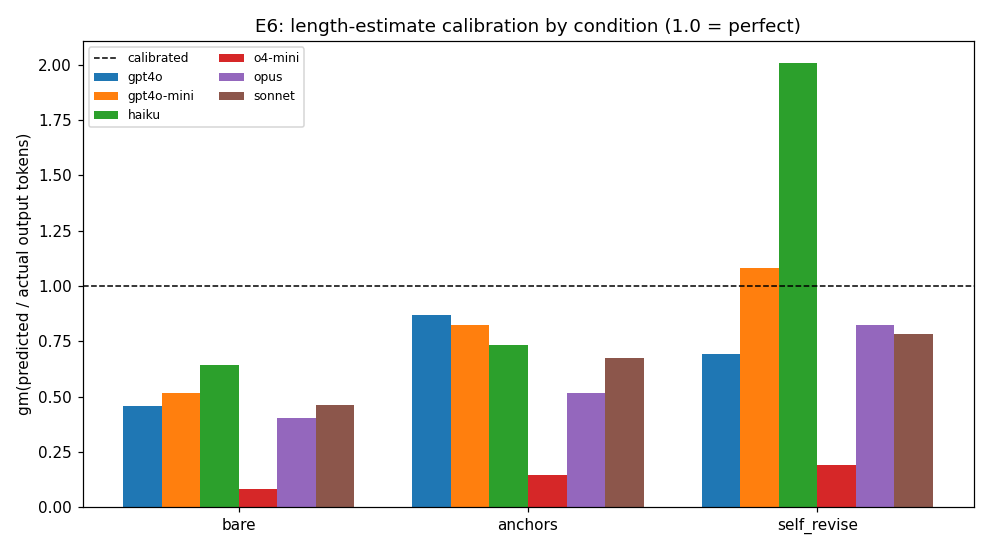
\includegraphics[width=0.66\textwidth]{e6-length-bias/ratio_by_condition.png}
\caption{E6: calibration (predicted/actual output tokens) by condition and model; dashed line is
perfect calibration. Self-revision pulls strong models to $\approx$1.0 but overshoots haiku and
fails to move o4-mini.}
\label{fig:e6}
\end{figure}

\paragraph{Verdict.} Largely supported. Target~1 (length self-estimation) is nearly free for
non-reasoning models via a fitted in-context correction; fine-tuning effort should be reserved
for the reasoning-model hidden-token problem, the one place in-context fixes fail.

\section{E10 --- Reasoning-model hidden-token probe}
\label{sec:e10}
\textbf{Hypothesis.} A reasoning model is blind to its own reasoning cost: it cannot predict how
much internal reasoning a problem needs ($\rho\approx 0$). This is the boundary E1, E2, E5, E6 all
isolated.

\paragraph{Setup.} 14 short-answer problems across a reasoning-difficulty gradient (all with a
one-token-ish final answer, so the variable is internal reasoning, not output). Per (model
$\times$ task $\times$ 3): \textbf{pre\_tokens} (estimate, without solving, how many internal
reasoning tokens it will need), \textbf{pre\_effort} (rate 1--10 how much thinking it needs), and
the solve, recording \emph{actual} \code{reasoning\_tokens} from usage. Models: o4-mini, gpt5 ---
the OpenAI reasoning models whose \code{reasoning\_tokens} vary with difficulty and are exposed
(gpt5.2 does not reason by default, excluded). 252 calls; actual reasoning spans 0--4757 tokens.

\paragraph{Results (Table~\ref{tab:e10}, Fig.~\ref{fig:e10}).} \textbf{The hypothesis is wrong,
and the truth is more interesting.} Reasoning models have strong \emph{ordinal} awareness of their
own reasoning cost but no \emph{magnitude} calibration. The 1--10 effort rating tracks actual
reasoning tokens well (pooled $\rho\,0.77$, ordering 0.90; gpt5 $\rho\,0.91$). But token-count
estimates are off $\sim$5--6$\times$ (gm 0.17--0.24), gpt5 frequently \emph{refuses} to give a
number (parseable for only 8/14 tasks, and wildly inconsistent when it does), and both models
badly under-rate the extreme: the hardest task ($\sim$4000+ reasoning tokens, 5--10$\times$ the
next) drew an effort rating of only 3/10.

\begin{table}[h]
\centering
\caption{E10: predicting one's own reasoning cost ($\rho$ vs actual \code{reasoning\_tokens}).}
\label{tab:e10}
\begin{tabular}{@{}llccc@{}}
\toprule
model & predictor & $\rho$ vs actual & ordering acc. & n \\
\midrule
gpt5    & effort 1--10    & \textbf{0.908} & 0.943 & 14 \\
o4-mini & token estimate  & 0.796 & 0.837 & 14 \\
o4-mini & effort 1--10    & 0.602 & 0.867 & 14 \\
gpt5    & token estimate  & 0.036 & 0.500 & 8$^{*}$ \\
\midrule
pooled  & effort 1--10    & \textbf{0.772} & 0.901 & 28 \\
pooled  & token estimate  & 0.403 & 0.668 & 22 \\
\bottomrule
\end{tabular}\\[2pt]
{\footnotesize $^{*}$gpt5 gave a parseable token number for only 8/14 tasks; its token-estimate
$\rho$ is on a thin self-selected subset and is not meaningful. Its effort rating is excellent.}
\end{table}

\begin{figure}[h]
\centering
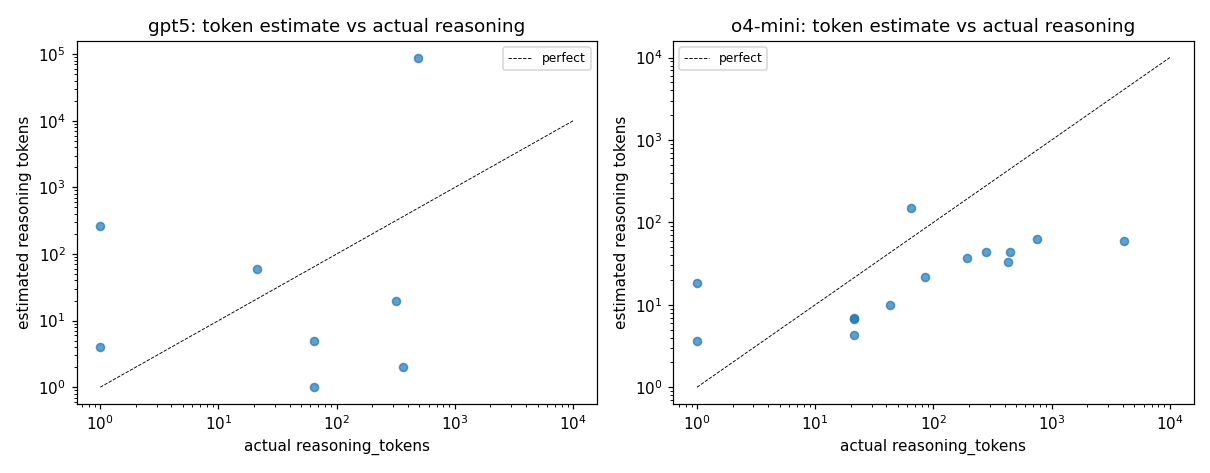
\includegraphics[width=0.92\textwidth]{e10-reasoning-tokens/estimate_vs_actual.png}
\caption{E10: predicted vs.\ actual reasoning tokens (log--log). Estimates cluster low and flat
relative to the wide actual range --- magnitude is uncalibrated even where ordering is good.}
\label{fig:e10}
\end{figure}

\paragraph{Why this refines the central boundary.} E1--E6 framed reasoning models as ``blind to
hidden reasoning.'' E10 sharpens that to \emph{magnitude}-blind, \emph{ordinally}-aware. Asked in
the right currency --- \emph{how hard is this for you?} not \emph{how many tokens?} --- the model
answers well. This is structurally the \emph{same} problem E6 fixed for output length: intact
ranking, broken scale. So the reasoning-model boundary is a tractable calibration target (a fitted
effort$\to$tokens map), not a fundamental wall --- the most optimistic update for the
``train-it-in'' direction.

\paragraph{Verdict.} Rejected, with a sharper replacement: reasoning models are ordinally aware of
their own reasoning effort ($\rho$ up to 0.91) but cannot calibrate its magnitude. \emph{Caveats:}
14 tasks, 2 models; gpt5 token refusals; reasoning effort is partly stochastic (a distribution,
not a point); Anthropic extended-thinking models untested.

\section{Statistical robustness}
\label{sec:ci}
95\% confidence intervals on the load-bearing headlines, via cluster bootstrap (\code{bootstrap\_ci.py})
resampling at the correct independent unit --- scenarios for E4, tasks for E5,
(model,task) units for E1/E2/E6 --- rather than individual rows, which would understate
uncertainty by ignoring the 3 correlated trials per unit. No new API calls.

\begin{center}
\begin{tabular}{@{}lll@{}}
\toprule
Statistic & Point & 95\% CI \\
\midrule
E4 correct rate --- no signal     & 0.494 & [0.485, 0.500] \\
E4 correct rate --- text          & 0.796 & [0.741, 0.854] \\
E4 correct rate --- harness clock & 0.956 & [0.917, 0.983] \\
E5 $\rho$ --- output control (C)  & $+0.788$ & [$+0.243$, $+0.835$] \\
E5 $\rho$ --- reasoning-decoupled (A) & $-0.067$ & [$-0.265$, $+0.199$] \\
E5 $\rho$ --- input-decoupled (B) & $-0.231$ & [$-0.495$, $-0.122$] \\
E1 $\rho$ (self-latency, overall) & 0.747 & [0.625, 0.835] \\
E2 $\rho$ --- seconds             & 0.657 & [0.499, 0.778] \\
E2 $\rho$ --- tokens              & 0.889 & [0.806, 0.938] \\
E6 gm --- bare                    & 0.37 & [0.29, 0.46] \\
E6 gm --- self\_revise            & 0.76 & [0.59, 0.95] \\
\bottomrule
\end{tabular}
\end{center}

\noindent The E4 ladder is cleanly separated. E5 confirms the proxy story: the control is robustly
positive while both decoupled families exclude positive calibration. E2's token-vs-second gap is
real but narrower than the points suggest (intervals nearly touch). \textbf{The wider intervals
(E5-C, E2) are limited by task/scenario count, not trial count} --- so the principled way to
tighten them is more scenarios (E7), not more trials, which is why we did not spend budget raising
N from 3.

\section{Synthesis}
\label{sec:synthesis}

The seven experiments tell one coherent story:
\begin{quote}\itshape
LLMs do not have an internal clock. They have an output-length estimator, and they respond to
elapsed time only when it is handed to them explicitly.
\end{quote}

\textbf{Self-perception (E1, E2, E5, E6, E10).} Apparent temporal self-awareness is output-length
anticipation. It proxies latency whenever latency is length-dominated (E1 $\rho$ up to 0.94; E2
token space $\rho\,0.89$), and collapses the instant latency hides in unseen reasoning or
prefill (E5 $\rho\approx 0$, constant estimates). The length undershoot is mostly an in-context
calibration error for non-reasoning models (E6 $0.37\to0.76$).

\textbf{Agency (E3, E4).} The same absence of a clock means agents act on elapsed time only when
it is explicit and loud: text timestamps get partway (E3/E4 0.80) because strong models can do
the arithmetic; an explicit sensor gets almost all the way (E4 0.96). The $0.49\to0.96$ gap is
largely a missing-sensor problem, not a missing-capability problem.

\textbf{The recurring boundary --- and its refinement (E10).} Across E1--E6 the reasoning model
was the exception: its latency hides in tokens it cannot see, so the length proxy (E1, E2, E5) and
every in-context fix (E6) failed on it. E10 probed this directly and \emph{softened} it: reasoning
models are not blind to their own reasoning --- their 1--10 effort rating tracks actual
reasoning-token expenditure well ($\rho$ up to 0.91, pooled 0.77) --- they only fail at magnitude
(token estimates off $\sim$5--6$\times$; gpt5 refuses them). So the boundary is \emph{ordinal
awareness intact, magnitude calibration broken} --- the same structure E6 fixed for output length,
hence a tractable calibration target rather than a wall. This is the most actionable update from
the follow-up round and de-risks the hardest case for the train-it-in direction.

\section{Recommendation and next experiments}
\label{sec:next}

Two framings are on record and are complementary, not exclusive:
\begin{itemize}
  \item \textbf{``Give it a sensor''} (\code{SUMMARY.md}): E4's harness clock is a cheap,
  deployable win. Treat it as the \emph{ceiling}.
  \item \textbf{``Train it in''} (\code{direction-train-it-in.md}): the absence of a clock is the
  reason to train the skill in. The research question is how much of the sensor's gap a model can
  \emph{internalize} from text alone --- internalization fraction
  $=(\text{trained}-\text{base})/(\text{ceiling}-\text{base})$.
\end{itemize}

A note on trainability, corrected from an earlier overstatement: predicting wall-clock seconds is
\emph{not} ill-posed within a \emph{fixed} environment. E1's latency CV of 0.04--0.14 shows the
seconds target is reproducible there; the constants (sec/token, overhead) are absorbed by
in-environment post-training. Only the \emph{cross-environment} target (from the prompt alone) is
ill-posed.

\paragraph{Experiments (detail in \code{experiments.md}).}
\begin{itemize}
  \item \textbf{E10 --- done} (\S\ref{sec:e10}): the reasoning-model boundary is ordinal-aware /
  magnitude-blind, hence a tractable calibration target. This was the cheap, high-value next step
  and it has been run.
  \item \textbf{E7} --- harden + scale E3: drop the stated staleness rule, add multi-turn, scale
  to $\sim$200 scenarios with held-out families. Prerequisite for E8.
  \item \textbf{E8} --- internalization: SFT (LoRA) a weak and a strong model on text-timestamp
  transcripts; report the internalization fraction per model (prediction: highest for weak
  models). The flagship of the train-it-in direction.
  \item \textbf{E9} --- sensor-format ablation: which representation (absolute / elapsed /
  relative / countdown) carries E4's lift.
\end{itemize}

\section{Limitations and process notes}
\label{sec:process}

\paragraph{Scientific limitations.}
\begin{itemize}
  \item \textbf{Small N} (3 trials; 9--14 tasks / scenarios). Trends are clear; tails are thin.
  Headline numbers now carry 95\% bootstrap CIs (\S\ref{sec:ci}); the limiting factor on the
  wider ones is task/scenario count, not trials.
  \item \textbf{Regime-specificity} (E1, E2, E6 use output-length--dominated tasks by design;
  E5 is the explicit decoupling check).
  \item \textbf{Forced one-word decisions} (E3, E4) and integer-second estimates (E1) are lower
  bounds on capability.
  \item \textbf{Stated thresholds} (E3, E4) isolate the sensor from threshold knowledge; absolute
  accuracies are optimistic, between-condition contrasts are the result.
  \item \textbf{Cost-estimate dollars} in each report are token-count $\times$ approximate prices,
  not billed amounts; total study spend was well within budget ($\sim$\$10 of a \$50+\$50 cap).
\end{itemize}

\paragraph{Process notes (so the next run avoids these).}
\begin{itemize}
  \item \textbf{Concurrent-writer bug.} Orchestration relaunched \code{run.py} while an earlier
  instance was still alive; both passed \code{load\_done()} and produced 492 duplicate rows in
  E4 (the E5/E6 driver hit the same race transiently but dedups every loop). Root cause: append
  + \code{load\_done()} is not concurrency-safe. Mitigation: single writer per experiment, and
  \code{dedup.py} before analysis. A file lock or a single coordinator is the proper fix.
  \item \textbf{Relative interpreter paths.} \code{.venv/bin/python} breaks inside a
  \code{cd}-subshell (exit 127); use the absolute interpreter path in scripts.
  \item \textbf{Background-job lifetime.} Long collections (slow reasoning models) outlived the
  job runner and were killed; \code{\_driver\_e5e6.py} is a self-healing driver that dedups and
  relaunches any died collection until expected counts are reached.
\end{itemize}

\appendix
\section{File manifest}
\label{app:manifest}
\begin{longtable}{@{}ll@{}}
\toprule
Path & Contents \\
\midrule
\endhead
\code{research-notes.md}        & Literature notes and reading list (seed doc) \\
\code{experiments.md}           & Full E1--E10 plan and status \\
\code{SUMMARY.md}               & Cross-experiment synthesis and recommendation \\
\code{direction-train-it-in.md} & Counterpoint ``train-it-in'' research direction \\
\code{common.py}                & Shared LLM-call helper (roster, timing, retries) \\
\code{dedup.py}                 & Canonicalize \code{results.jsonl} by logical key \\
\code{bootstrap\_ci.py}         & 95\% cluster-bootstrap CIs for headline statistics \\
\code{\_driver\_e5e6.py}        & Self-healing overnight collection driver \\
\code{requirements.txt}         & Pinned Python dependencies \\
\code{eN-*/run.py}              & Data collection (resumable) \\
\code{eN-*/analyze.py}          & Statistics + figures from \code{results.jsonl} \\
\code{eN-*/results.jsonl}       & Raw per-call data (canonical, deduped) \\
\code{eN-*/REPORT.md}           & Self-contained per-experiment findings \\
\code{eN-*/*.png}               & Figures \\
\code{e4-harness-clock/NOTES.md}& Debugging log (opus temperature, dedup) \\
\bottomrule
\end{longtable}

\section{Experiment summary table}
\label{app:summary}
\begin{center}
\begin{tabular}{@{}llp{6.2cm}@{}}
\toprule
Exp & Calls & One-line result \\
\midrule
E1 & 648  & Self-latency calibration is a length proxy ($\rho$ up to 0.94); not 4--7$\times$ overshoot. \\
E2 & 864  & Token space beats seconds ($\rho\,0.89$ vs $0.66$); $\sim$2$\times$ length undershoot. \\
E3 & 810  & Timestamp-sensitivity graded by model strength (opus 1.00 $\to$ haiku 0.56). \\
E4 & 1620 & Harness clock 0.96 $>$ text 0.80 $>$ none 0.49. \\
E5 & 450  & Calibration collapses when latency is decoupled ($\rho\approx 0$); confirms length proxy. \\
E6 & 720  & Self-revision closes the undershoot $0.37\to0.76$ (non-reasoning models). \\
E10 & 252 & Reasoning models are ordinally aware (effort $\rho$ up to 0.91) but magnitude-blind. \\
\bottomrule
\end{tabular}
\end{center}

\end{document}
